\documentclass[11pt]{article}
\usepackage[margin={.6in, .6in}]{geometry} 
\usepackage{grid-system, graphicx}
\usepackage{cmbright}
\usepackage{grffile}
\usepackage{wrapfig}

\newcommand{\plotpath}[1]{{../plots_oberbayern_NEWDATA_MAXPOP5000/#1}.pdf}
\newcommand{\plotwidth}{\textwidth}
\newcommand{\plotrow}[2]{\begin{Row}
		\begin{Cell}{1}%
%			\centering
			\includegraphics[width=\plotwidth]{\plotpath{#1}}%
		\end{Cell}%
		\begin{Cell}{1}%
			\if\relax\detokenize{#2}\relax
			\else
%			\centering
			\includegraphics[width=\plotwidth]{\plotpath{#2}}%
			\fi
		\end{Cell}
	\end{Row}
}
\newcommand{\plot}[1]{\begin{figure}[h]
		\includegraphics[width=0.5\textwidth]{\plotpath{#1}}%
\end{figure}}

\setcounter{section}{-1}

\begin{document}

\begin{center}
	\Huge \textbf{Statistischer Vergleich Engelsbergs mit Gemeinden im Regierungsbezirk Oberbayern mit höchstens 5000 Einwohnern}
\end{center}
\pagebreak

\renewcommand{\contentsname}{Inhalt}
\tableofcontents

\pagebreak
\section{Erläuterungen}
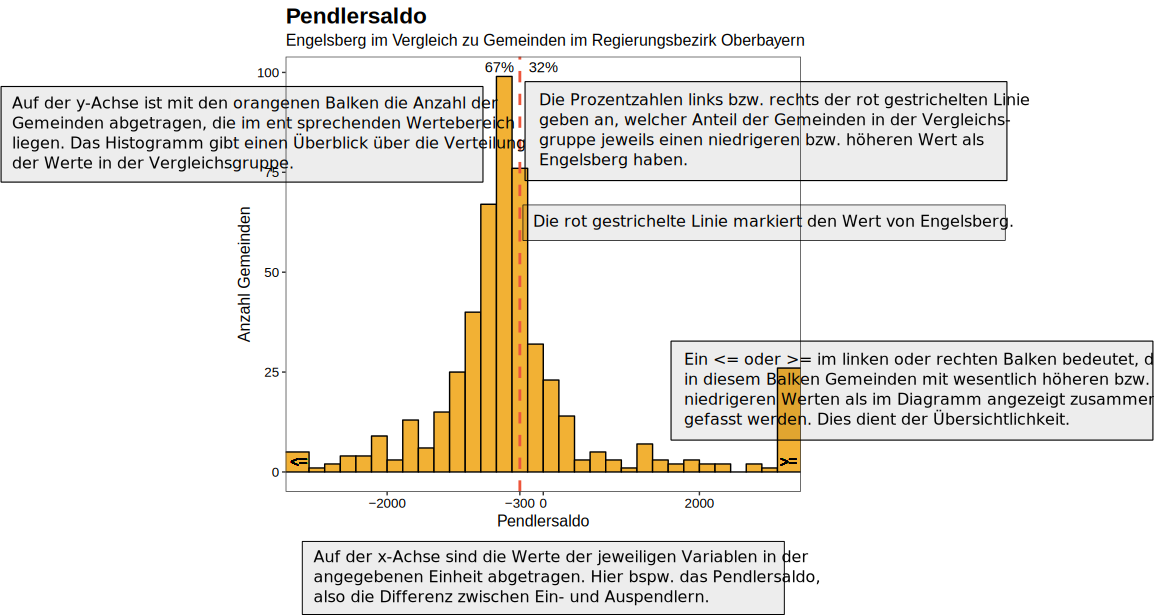
\includegraphics[width=\textwidth]{../plot_explanations}

\vfill

\subsection*{Bevölkerung}
Dieser Vergleich ist auf Gemeinden mit einer Bevölkerung von 5000 oder niedriger beschränkt, um eine bessere Vergleichbarkeit mit Engelsberg zu gewährleisten. Allein die Darstellung der Gesamtbevölkerung (Bevölkerung 2015, Seite \pageref{plot:bevoelkerung.insgesamt}) basiert auf allen Gemeinden.

\subsection*{Quellenangaben}
Alle Diagramme basieren auf verarbeiteten Daten aus Gemeindedaten für Bayern 2018. Ausgewählte statistische Daten für Regierungsbezirke, kreisfreie Städte und Landkreise, Gemeinden und Verwaltungsgemeinschaften sowie Regionen, \textit{Bayerisches Landesamt für Statistik} (2018).

Sofern nicht anders angegeben, beruhen alle Daten auf dem \textbf{Kalenderjahr 2017}.

\pagebreak

\section{Eine junge und finanzstarke Gemeinde}

\paragraph{Die Bevölkerung von Engelsberg und seine Entwicklung: 24 Jahre lang starke Zunahme, dann Stagnation}
Im Vergleich der oberbayerischen Gemeinden mit einer Bevölkerung von höchstens 5000 Einwohnern liegt die Einwohnderdichte Engelsbergs etwa im Durchschnitt: 59\% der Gemeinden haben mehr Einwohner pro Fläche. Die Einwohnerzahl von Engelsberg hat in 24 Jahren – zwischen 1987 und 2011 – immer wieder zugenommen; dagegen gab es nach 2011 keinerlei Veränderungen mehr.
Dass dieser Zuwachs bis 2011 enorm war, zeigt der Vergleich:  Knapp 90\% der Gemeinden sind in diesen 30 Jahren weniger gewachsen und nur 12\% haben stärker zugenommen als Engelsberg. Seit 2017 drehte sich das Blatt:  2017 zogen 160 Leute nach Engelsberg und 204 verließen die Gemeinde. Deutlich wird dies auch beim Wanderungsgewinn (Differenz von Menschen, die innerhalb eines Jahres einwandern und denen, die in diesem Zeitraum auswandern): Hier liegen 99 der Gemeinden höher als Engelsberg.

\vspace{1em}
\addcontentsline{toc}{subsection}{Bevölkerung insgesamt}
\addcontentsline{toc}{subsection}{Bevölkerungsdichte}
\label{plot:bevoelkerung.insgesamt}
\plotrow{bevoelkerung.insgesamt}{bevoelkerung.je_km2}

\addcontentsline{toc}{subsection}{Bevölkerungsveränderung im Vgl. zu 1987}
\addcontentsline{toc}{subsection}{Bevölkerungsveränderung im Vgl. zu 2011}
\plotrow{bevoelkerung.veraenderung.vs.1987}{bevoelkerung.veraenderung.vs.2011}

\addcontentsline{toc}{subsection}{Bevölkerungsbewegung: Wanderungsgewinn}
\addcontentsline{toc}{subsection}{Bevölkerung: Altersstruktur}
\plotrow{bevoelkerung.bewegung.wanderungsgewinn}{altersstruktur}

\section{Altersstruktur}
\paragraph{Engelsberg ist eine junge Gemeinde}
Engelsberg ist eine relativ junge Gemeinde, denn hier ist im Vergleich zu anderen Gemeinden der Anteil von jungen Menschen etwas höher. In den jüngsten fünf Altersgruppen sind die Zahlen durchweg etwas höher als im oberbayerischen Durchschnitt; in den drei älteren Altersgruppen durchweg etwas niedriger.

\section{Die Flächen von Engelsberg}
\paragraph{Viel freies Land mit viel Landwirtschaft}
Der Anteil der Gebäude- und Freiflächen an der Gesamtfläche (=Flächen mit Gebäuden und baulichen Anlagen sowie unbebaute Flächen (Freiflächen), die Zwecken der Gebäude untergeordnet sind) ist in Engelsberg ist knapp 2\% ziemlich gering: Knapp zwei Drittel der Gemeinden haben hier einen höheren Anteil. Dasselbe gilt für den Anteil der Betriebsfläche (unbebaute Fläche, die überwiegend gewerblich, industriell oder zur Ver- und Entsorgung genutzt werden, einschließlich der Flächen für Gebäude von geringem Wert) mit etwa 0,5\%. Dagegen nimmt die Landwirtschaftsfläche einen sehr großen Teil ein: Mit knapp 70\% liegt Engelsberg hier weit vorne – nur 15\% aller Gemeinden haben hier einen höheren Wert. Dagegen ist der Waldanteil im Engelsberger Gebiet relativ gering: Mit gut 20\% haben zwei Drittel der Gemeinden mehr Waldfläche. Auch bei der Erholungsfläche (Flächen, die vorherrschend dem Sport, der Erholung oder dazu dienen, Tiere oder Pflanzen zu zeigen) liegt Engelsberg am unteren Ende der Statistik: Hier haben 84\% der Gemeinden höhere Werte.

\vspace{1em}
\addcontentsline{toc}{subsection}{Anteil Gebäude- und Freifläche}
\addcontentsline{toc}{subsection}{Anteil Betriebsfläche}
\plotrow{gebfreifl.rel}{betrfl.rel}

\addcontentsline{toc}{subsection}{Anteil Landwirtschaftsfläche}
\addcontentsline{toc}{subsection}{Anteil Waldfläche}
\plotrow{landwfl.rel}{waldfl.rel}

\addcontentsline{toc}{subsection}{Anteil Erholungsfläche}
\plotrow{erholfl.rel}{}

\section{Wohnen in Engelsberg}
\paragraph{Durchschnittlich viele Wohnungen und Baugenehmigungen}
Beim Wohnungsbestand liegt Engelsberg in der Mitte der oberbayerischen Statistik: 43\% der Gemeinden haben mehr Wohnungen. Ähnliches gilt für erteilte Baugenehmigungen: Hier lagen 52\% der Gemeinden über den Zahlen von Engelsberg.

\paragraph{Kinderbetreuung und Bildung: Wenige Kindertagesstätten und viele Schüler}
Bei den Kindertageseinrichtungen weist Engelsberg nur einen geringen Anteil im oberbayerischen Vergleich auf: 78\% der Gemeinden haben mehr Plätze pro Einwohner. Dagegen hat die Gemeinde Engelsberg relativ viele Schüler (hier zeigt es sich wieder, dass Engelsberg eine junge Gemeinde ist): Mit 4\% Anteil an der Bevölkerung haben fast zwei Drittel der Gemeinden weniger Schüler.

\vspace{1em}
\addcontentsline{toc}{subsection}{Wohnungsbestand}
\addcontentsline{toc}{subsection}{Baugenehmigungen für Wohnungen}
\plotrow{bauwohn.bestand_wohnungen.insgesamt}{bauwohn.baugenehmigungen.wohnungen}

\addcontentsline{toc}{subsection}{Kindertagesplätze}
\addcontentsline{toc}{subsection}{Schüler}
\plotrow{bildung.kindertages.plaetze.pro100}{schueler.insg.rel}



\section{Landwirtschaft und Umwelt}
\paragraph{An der Spitze in Oberbayern liegt Engelsberg...} mit seinen 72  Land- und forstwirtschaftlichen Betrieben: nur 9\% der Gemeinden haben hier mehr.
Womöglich in Zusammenhang damit steht der im Vergleich hohe Wasserverbrauch  mit 139 Litern pro Person und Tag. Nur 13\% der Gemeinden verbrauchen mehr Wasser.

\vspace{1em}
\addcontentsline{toc}{subsection}{Land- und forstwirtschaftliche Betriebe}
\addcontentsline{toc}{subsection}{Wasserverbrauch pro Kopf}
\plotrow{landforst.betriebe_von_flaeche_ha.insgesamt}{umwelt.wasser_pro_kopf_verbrauch}

\section{Erwerb, Einkommen und Soziales}
\paragraph{Viele Beschäftigte – mehr Auspendler – relativ hohe Einkünfte}
Mit 760 Personen, die in Engelsberg arbeiten, ist die Beschäftigungszahl relativ hoch im Vergleich: nur 20\% der Gemeinden liegen darüber.
Darunter fahren exakt drei Viertel nach Engelsberg, um dort zu arbeiten – die Einpendler. Ebenfalls eine relativ hohe Zahl – 82\% sind außerhalb beschäftigt – die Auspendler. 
Zum Vergleich: In 37\% der Gemeinden ist die Zahl der Einpendler noch höher.
Genau das Gegenteil zeigt sich bei den Auspendlern: 82\% der Engelsberger Arbeitnehmer verlassen den Ort, um woanders zu arbeiten, was sich so in ganz Oberbayern widerspiegelt: Nur in 19\% der Gemeinden ist dieser Anteil geringer – also die  meisten oberbayerischen Gemeinden haben eine hohe Zahl von Auspendlern.
Diese Zahlen werden  beim Pendlersaldo (gibt an, ob mehr Arbeitskräfte regelmäßig von ihrem Wohnort zum Arbeiten in die Gemeinde kommen, oder mehr Gemeindebürger sie regelmäßig verlassen, da ihr Arbeitsplatz außerhalb der Region liegt) deutlich: Hier haben 70 \% der Gemeinden eine positivere  Bilanz. 
 

\addcontentsline{toc}{subsection}{Beschäftigte am Arbeitsort}
\addcontentsline{toc}{subsection}{Beschäftigte am Arbeitsort, darunter Einpendler}
\plotrow{erwerb.sozialverspfl_beschaeftigte_am_arbeitsort.insgesamt}{erwerb.sozialverspfl_beschaeftigte_am_arbeitsort.darunter_einpendler.prozent}



\pagebreak
Bei der Lohn- und Einkommenssteuer (Bruttolohn je Arbeitnehmer, von 2014) liegt Engelsberg genau in der Mitte von Oberbayern: 48\% der Gemeinden haben hier einen höheren Wert.
Dass die Engelsberger relativ hohe Einkünfte im statistischen Vergleich haben – sie betragen im Schnitt über 38 000 Euro - zeigen diese Zahlen: Bei den Gesamtbeträgen aller Einkünfte (2014) können sich in nur 37\% anderer Gemeinden  die Bewohner über noch mehr Geld freuen.
Mit leicht 1\% Anteil an der Bevölkerung ist die Zahl der Sozialhilfeempfänger in Engelsberg im Vergleich leicht überdurchschnittlich: 60\% der Gemeinden haben hier weniger Sozialhilfeempfänger.

\vspace{1em}
\addcontentsline{toc}{subsection}{Beschäftigte am Wohnort, darunter Auspendler}
\addcontentsline{toc}{subsection}{Pendlersaldo}
\plotrow{erwerb.sozialverspfl_beschaeftigte_am_wohnort.darunter_auspendler.prozent}{erwerb.pendlersaldo}



\addcontentsline{toc}{subsection}{Bruttolohn je Arbeitnehmer}
\addcontentsline{toc}{subsection}{Lohn- und Einkommensteuer: Gesamtbetrag der Einkünfte}
\plotrow{lohneinksteuer.bruttolohn.je_arbeitnehmer}{lohneinksteuer.gesamtbetrag_einkuenfte.insgesamt}

\addcontentsline{toc}{subsection}{Lohn- und Einkommensteuer: Einkünfte je Steuerpflichtiger}
\addcontentsline{toc}{subsection}{Sozialhilfeempfänger}
\plotrow{lohneinksteuer.gesamtbetrag_einkuenfte.je_steuerpfl}{sozialhilfe_empf.insg.rel}

\pagebreak
\section{Kommunale Finanzen}
\paragraph{Eine finanzstarke Gemeinde}
Engelsberg steht im oberbayerischen Vergleich finanziell sehr gut da. Dies zeigen diese Zahlen:
Bei der Grundsteuer A (für landwirtschaftliche Betriebe) liegt Engelsberg im oberbayerischen Vergleich mit an der Spitze – vermutlich durch seine vielen landwirtschaftlichen Betriebe. Hier verzeichnen nur 10\% der Gemeinden höhere Einnahmen durch die Grundsteuer A.
Auch bei der Grundsteuer B (für bebaute und unbebaute Grundstücke) liegt Engelsberg etwa im oberen Drittel: 39\% der Gemeinden nehmen mehr Grundsteuer B ein.
Insgesamt hat Engelsberg durch die Grundsteuern im Vergleich relativ hohe Einnahmen.

\vspace{1em}
\addcontentsline{toc}{subsection}{Gemeindesteuereinnahmen: Grundsteuer A}
\addcontentsline{toc}{subsection}{Gemeindesteuereinnahmen: Grundsteuer B}
\plotrow{kommunale_finanzen.gemeindesteuereinnahmen.darunter.grundsteuer.a}{kommunale_finanzen.gemeindesteuereinnahmen.darunter.grundsteuer.b}

\addcontentsline{toc}{subsection}{Steuereinnahmen insgesamt}
\addcontentsline{toc}{subsection}{Gemeindesteuereinnahmen insgesamt}
\plotrow{kommunale_finanzen.steuereinnahmen_insgesamt}{kommunale_finanzen.gemeindesteuereinnahmen.insgesamt}

\pagebreak
Bei den Gesamtsteuerannahmen mit 1336 Euro je Einwohner liegt Engelsberg an der Spitze: nur 9\% alle Gemeinden haben einen noch besser gefüllten Geldsäckel. Bei den Gemeindesteuereinnahmen mit dreieinhalb Millionen Euro liegt Engelsberg ebenfalls im oberen Bereich der Statistik: Nur 18\% der Gemeinden haben hier eine höhere Zahl.
Dies zeigt sich auch bei der Steuereinnahmekraft (eine Kenngröße, mit deren Hilfe Städte und Gemeinden mit unterschiedlichen Realsteuerhebesätzen -- Grundsteuer A/B, Gewerbesteuer -- vergleichbarer gemacht werden sollen): Nur 9\% der Gemeinden erreichen hier höhere Werte.
Genau so spiegeln sich die Finanzen bei der Realsteueraufbringungskraft wider (sie errechnet sich für die jeweilige Steuerart einer Gemeinde (Gewerbesteuer, Grundsteuer A und B) über eine bestimmte Formel): Auch hier nimmt Engelsberg in Oberbayern einen Spitzenplatz ein: Nur 8\% der Gemeinden erreichen bessere Zahlen pro Einwohner.

\vspace{1em}
\addcontentsline{toc}{subsection}{Steuereinnahmekraft je Einwohner}
\addcontentsline{toc}{subsection}{Realsteueraufbringungskraft}
\plotrow{kommunale_finanzen.steuereinnahmekraft.je_einwohner}{kommunale_finanzen.realsteueraufbringungskraft}

%\section{Bevölkerung}
%	\addcontentsline{toc}{subsection}{Bevölkerung insgesamt}
%	\addcontentsline{toc}{subsection}{Bevölkerungsdichte}
%	\label{plot:bevoelkerung.insgesamt}
%	\plotrow{bevoelkerung.insgesamt}{bevoelkerung.je_km2}
%	
%	\addcontentsline{toc}{subsection}{Bevölkerungsveränderung im Vgl. zu 1987}
%	\addcontentsline{toc}{subsection}{Bevölkerungsveränderung im Vgl. zu 2011}
%	\plotrow{bevoelkerung.veraenderung.vs.1987}{bevoelkerung.veraenderung.vs.2011}
%	
%	\addcontentsline{toc}{subsection}{Bevölkerungsbewegung: Zugezogene}
%	\addcontentsline{toc}{subsection}{Bevölkerungsbewegung: Fortgezogene}
%	\plotrow{bevoelkerung.bewegung.zugezogene}{bevoelkerung.bewegung.fortgezogene}
%	
%	\addcontentsline{toc}{subsection}{Bevölkerungsbewegung: Wanderungsgewinn}
%	\addcontentsline{toc}{subsection}{Bevölkerung: Altersstruktur}
%	\plotrow{bevoelkerung.bewegung.wanderungsgewinn}{altersstruktur}
%
%\section{Flächen}
%	\addcontentsline{toc}{subsection}{Anteil Gebäude- und Freifläche}
%	\addcontentsline{toc}{subsection}{Anteil Betriebsfläche}
%	\plotrow{gebfreifl.rel}{betrfl.rel}
%	
%	\addcontentsline{toc}{subsection}{Anteil Landwirtschaftsfläche}
%	\addcontentsline{toc}{subsection}{Anteil Waldfläche}
%	\plotrow{landwfl.rel}{waldfl.rel}
%	
%	\addcontentsline{toc}{subsection}{Anteil Erholungsfläche}
%	\plotrow{erholfl.rel}{}
%
%\section{Wohnen}
%	\addcontentsline{toc}{subsection}{Wohnungsbestand}
%	\addcontentsline{toc}{subsection}{Baugenehmigungen für Wohnungen}
%	\plotrow{bauwohn.bestand_wohnungen.insgesamt}{bauwohn.baugenehmigungen.wohnungen}
%
%\section{Kinderbetreuung und Bildung}
%	\addcontentsline{toc}{subsection}{Kindertagesplätze}
%	\addcontentsline{toc}{subsection}{Schüler}
%	\plotrow{bildung.kindertages.plaetze.pro100}{schueler.insg.rel}
%
%\section{Landwirtschaft und Umwelt}
%	\addcontentsline{toc}{subsection}{Land- und forstwirtschaftliche Betriebe}
%	\addcontentsline{toc}{subsection}{Wasserverbrauch pro Kopf}
%	\plotrow{landforst.betriebe_von_flaeche_ha.insgesamt}{umwelt.wasser_pro_kopf_verbrauch}
%
%\section{Erwerb, Einkommen und Soziales}
%	\addcontentsline{toc}{subsection}{Beschäftigte am Arbeitsort}
%	\addcontentsline{toc}{subsection}{Beschäftigte am Arbeitsort, darunter Einpendler}
%	\plotrow{erwerb.sozialverspfl_beschaeftigte_am_arbeitsort.insgesamt}{erwerb.sozialverspfl_beschaeftigte_am_arbeitsort.darunter_einpendler.prozent}
%	
%	\addcontentsline{toc}{subsection}{Beschäftigte am Wohnort, darunter Auspendler}
%	\addcontentsline{toc}{subsection}{Pendlersaldo}
%	\plotrow{erwerb.sozialverspfl_beschaeftigte_am_wohnort.darunter_auspendler.prozent}{erwerb.pendlersaldo}
%	
%	\addcontentsline{toc}{subsection}{Bruttolohn je Arbeitnehmer}
%	\addcontentsline{toc}{subsection}{Lohn- und Einkommensteuer: Gesamtbetrag der Einkünfte}
%	\plotrow{lohneinksteuer.bruttolohn.je_arbeitnehmer}{lohneinksteuer.gesamtbetrag_einkuenfte.insgesamt}
%	
%	\addcontentsline{toc}{subsection}{Lohn- und Einkommensteuer: Einkünfte je Steuerpflichtiger}
%	\addcontentsline{toc}{subsection}{Sozialhilfeempfänger}
%	\plotrow{lohneinksteuer.gesamtbetrag_einkuenfte.je_steuerpfl}{sozialhilfe_empf.insg.rel}
%
%\section{Kommunale Finanzen}
%	\addcontentsline{toc}{subsection}{Gemeindesteuereinnahmen: Grundsteuer A}
%	\addcontentsline{toc}{subsection}{Gemeindesteuereinnahmen: Grundsteuer B}
%	\plotrow{kommunale_finanzen.gemeindesteuereinnahmen.darunter.grundsteuer.a}{kommunale_finanzen.gemeindesteuereinnahmen.darunter.grundsteuer.b}
%	
%	\addcontentsline{toc}{subsection}{Steuereinnahmen insgesamt}
%	\addcontentsline{toc}{subsection}{Gemeindesteuereinnahmen insgesamt}
%	\plotrow{kommunale_finanzen.steuereinnahmen_insgesamt}{kommunale_finanzen.gemeindesteuereinnahmen.insgesamt}
%	
%	\addcontentsline{toc}{subsection}{Steuereinnahmekraft je Einwohner}
%	\addcontentsline{toc}{subsection}{Realsteueraufbringungskraft}
%	\plotrow{kommunale_finanzen.steuereinnahmekraft.je_einwohner}{kommunale_finanzen.realsteueraufbringungskraft}

\end{document}

%\begin{Row}
%	\begin{Cell}{1}
%		\includegraphics[width=\plotwidth]{\plotpath{}}
%	\end{Cell}
%	\begin{Cell}{1}
%		\includegraphics[width=\plotwidth]{\plotpath{}}
%	\end{Cell}
%\end{Row}
